 % AUTHOR: Diego Sarceno
% Last Update: 11.07.2020

\documentclass[11pt, spanish, letterpage]{article} %tipo de documento

\usepackage[letterpaper]{geometry} %margenes
\geometry{verbose,tmargin=2.5cm,bmargin=2.5cm,lmargin=2cm,rmargin=2cm}
\usepackage{amsmath,amsthm,amssymb} %modos matemáticos y  simbolos
\usepackage{latexsym,amsfonts} %simbolos matematicos
\usepackage{cancel} %hacer la linea que cancela las ecuaciones
\usepackage[spanish, es-noshorthands]{babel} %comandos en español y cambia el cuadro por la tabla
\decimalpoint %cambia las comas por puntos decimal
\usepackage[utf8]{inputenc} %caracteristicas del español
\usepackage{physics} %Simbolos fisicos
\usepackage{array} %mejores formatos de tabla
\parindent =0cm %sangria
\usepackage{graphicx} %graficas e imagenes
\usepackage{mathtools}
\usepackage[framemethod=TikZ]{mdframed}%Entornos talegas
\usepackage[colorlinks = true,
			linkcolor = blue,
			citecolor = black,
			urlcolor = blue]{hyperref}%formato de los links y URL's
\usepackage{multicol} %varias columnas
\usepackage{enumerate} %enumeraciones
\usepackage{pgf,tikz,pgfplots} %documentos en formato tikz
\usepackage{mathrsfs} %letras chingonas (transformada de laplace)
\usepackage{subfigure} %varias figuras seguidas
\usepackage[square,numbers]{natbib} %bibliografias
\usepackage[nottoc]{tocbibind}
\bibliographystyle{plainnat}
\usetikzlibrary{arrows, babel, calc}
\usepackage{tabulary}
\usepackage{multirow} %ocupar varias filas en una tabla
\usepackage{fancybox} %recuadros talegas
\usepackage{float} %ubicar graficas
\usepackage{color}
\usepackage{comment}
\usepackage{stackrel}
\usepackage{calligra}
\usepackage{lipsum} % texto de relleno
\usepackage{cite}
\usepackage{circuitikz} % crear circuitos
\usepackage{listings} % permite el ingreso de codigo
\usepackage{longtable}
%\usepackage{showframe}
%\usepackage{LobsterTwo}
% NEW PACKAGES
\usepackage{makeidx}
\usepackage{authblk} % para la manipulación de autores y afiliación
\usepackage{booktabs}
\usepackage{colortbl}
\usepackage{bbold}
\usepackage{dsfont}
\usepackage{tensor}
\usepackage{colortbl}
\usepackage{amsbsy}
\usepackage[draft,inline,nomargin]{fixme} \fxsetup{theme=color}

%This defines my comments
\definecolor{mycolor}{RGB}{0,0,250}
\FXRegisterAuthor{ds}{sds}{\color{mycolor}DS}


\usepackage{pdfpages}
\setlength{\parindent}{1cm} %sangria

%%%%%%%%%%%%%%%%%%%%%%%%%%%%%%%%%%%%%%%%%%%%%%%%%%%%%%%%%%%
\lstset{basicstyle=\ttfamily,breaklines=true}
\lstset{numbers=left, numberstyle=\tiny, stepnumber=1, numbersep=6pt}
\lstset{emph={import,as,return,for,in,else,if,def,True,const,False,append}, emphstyle=\color{blue}, emph={[2]pKronecker},
emphstyle={[2]\color{violet}}, emph={[3]float,input,int,range,print,len,double},
emphstyle={[3]\color{violet}}}
\lstset{morecomment=[l][\color{gray!40}]{\#}, morestring=[b][\color{green!50!black}]"}
%%	Importe de archivo: \lstinputlisting[inputencoding=latin1]{'nombre del archivo'.py}
%%%%%%%%%%%%%%%%%%%%%%%%%%%%%%%%%%%%%%%%%%%%%%%%%%%%%%%%%%%
\setlength{\columnseprule}{0pt}
%-------------------------------------------------
%\newcommand{\N}{\mathbb{N}}
%\newcommand{\Z}{\mathbb{Z}}
%\newcommand{\Q}{\mathbb{Q}}
%\newcommand{\I}{\mathbb{I}}
%\newcommand{\R}{\mathbb{R}}
%\newcommand{\C}{\mathbb{C}} %Conjuntos numericos
%\newcommand{\F}{\mathbb{F}} %Campo Cualquiera
%\newcommand{\Pos}{\mathbb{P}} %Reales positivos

\def\do#1{\csdef{#1}{\mathbb{#1}}}
\docsvlist{N,Z,Q,I,R,C,F,P}


\newcommand{\Hilbert}{\mathcal{H}} % Espacio de Hilbert
\newcommand{\f}{\textit{f}} %f de funcion
\newcommand{\g}{\textit{g}}
\newcommand{\kernel}{\mathscr{N}} %kernel
\newcommand{\range}{\mathcal{R}} %range
\newcommand{\lagran}{\mathcal{L}} %lagrangiano
\newcommand{\laplace}{\mathscr{L}} %transformada de laplace, mapas lineales
\newcommand{\partition}{\mathfrak{z}} % función de partición
\newcommand{\M}{\mathcal{M}} %Matrices
\newcolumntype{E}{>{$}c<{$}} %entorno matematico en columnas de una tabla
\newcommand{\vi}{\boldsymbol{\hat{\imath}}}
\newcommand{\vj}{\boldsymbol{\hat{\jmath}}}
\newcommand{\vk}{\vu{k}}%vectores unitarios R3
\newcommand{\vr}{\hat{r}}
\newcommand{\vp}{\boldsymbol{\hat{\phi}}}
\newcommand{\vz}{\vu{z}}%vectores unitarios en cilindricas
\newcommand{\vaz}{\boldsymbol{\hat{\theta}}}%vectores unitarios en esféricas
\newcommand{\vx}{\vu{x}}%vectores
\newcommand{\vy}{\vu{y}}%vectores 
\newcommand\numberthis{\addtocounter{equation}{1}\tag{\theequation}}
\newcommand{\LI}{\lim _{h\longrightarrow 0}}
\newcommand{\SU}{\longrightarrow \sum _{n=0} ^{\infty}}
\newcommand{\QED}{\hfill {\qed}}
\newcommand{\cis}{\text{cis} \,}
% matrices de pauli
\newcommand{\pauli}[1]{\sigma _{#1}}
%----------------------------------------------------------
%----------------------------------------------------------


%-paquete para unidades en el sistema internacional
\usepackage[load=prefix, load=abbr, load=physical]{siunitx}
\newunit{\gram}{g }%gramos
\newunit{\velocity}{ \metre / \Sec }%unidades de velocidad sistema internacional
\newunit{\acceleration}{ \metre / \Sec^2 }%unidades de aceleracion sistema internacional
\newunit{\entropy}{ \joule / \kelvin }%unidades de entropia sistema internacional
%--definiendo constantes fisicas en el SI
\newcommand{\accgravity}{9.8 \metre / \Sec^2}
%---diferencial inexacta
\newcommand{\dbar}{\mathchar'26\mkern-12mu d}
%-------------------------END-------------------------------------
%------------------------Barra negra-------------------------------
\tikzset{
	warningsymbol/.style={
		rectangle,draw=black,
		fill=white,scale=1,
		overlay}}
\mdfdefinestyle{warning}{%
	hidealllines=true,leftline=true,
	skipabove=12,skipbelow=12pt,
	innertopmargin=0.4em,%
	innerbottommargin=0.4em,%
	innerrightmargin=0.7em,%
	rightmargin=0.7em,%
	innerleftmargin=1.7em,%
	leftmargin=0.7em,%
	middlelinewidth=.2em,%
	linecolor=black,%
	fontcolor=black,%
	firstextra={\path let \p1=(P), \p2=(O) in ($(\x2,0)+0.5*(0,\y1)$)
										node[warningsymbol] {$\mathcal{S}$};},%
	secondextra={\path let \p1=(P), \p2=(O) in ($(\x2,0)+0.5*(0,\y1)$)
										node[warningsymbol] {$\mathcal{S}$};},%
	middleextra={\path let \p1=(P), \p2=(O) in ($(\x2,0)+0.5*(0,\y1)$)
										node[warningsymbol] {$\mathcal{S}$};},%
	singleextra={\path let \p1=(P), \p2=(O) in ($(\x2,0)+0.5*(0,\y1)$)
										node[warningsymbol] {$\mathcal{S}$};},%
}
%%%%%%%%%%%%%%%%%%%%%%%%%%%%%%%%%%% Tema - BEGIN
\newtheoremstyle{Tema}% name of the style to be used
  {0mm}% measure of space to leave above the theorem. E.g.: 3pt
  {10mm}% measure of space to leave below the theorem. E.g.: 3pt
  {}% name of font to use in the body of the theorem
  {}% measure of space to indent
  {\bfseries}% name of head font
  {\newline}% punctuation between head and body
  {30mm}% space after theorem head
  {}% Manually specify head

\theoremstyle{Tema} \newtheorem{Tema}{Tema} %%%%% Template para Temas
\theoremstyle{Tema} \newtheorem{serie}{Serie}              %%%%%  Template para Series de ejercicios
\theoremstyle{Tema} \newtheorem{teorema}{Teorema}              %%%%%  Template para Teoremas
\theoremstyle{Tema} \newtheorem{pregunta}{Pregunta}              %%%%%  Template para Series de ejercicios
\theoremstyle{Tema} \newtheorem{ejercicio}{Ejercicio}    %%%%%  Template para Ejercicios
\theoremstyle{Tema} \newtheorem{ejemplo}{Ejemplo}    %%%%%  Template para Ejemplos
\theoremstyle{Tema} \newtheorem{solucion}{Solución}    %%%%%  Template para Soluciones
\theoremstyle{Tema} \newtheorem{problem}{Problema}    %%%%%  Template para Problema
\theoremstyle{Tema} \newtheorem{definicion}{Definición}    %%%%%  Template para Soluciones
\theoremstyle{Tema} \newtheorem{proposicion}{Proposición}    %%%%%  Template para Soluciones
\theoremstyle{Tema} \newtheorem{lema}{Lema}    %%%%%  Template para Soluciones
\theoremstyle{Tema} \newtheorem{reto}{Reto}    %%%%%  Template para Reto
%-------------------------END-------------------------------------


%%%%%%%%%%%%%%%%%%%%%%%%%%%%%%%%%%%%%%%%%%%%%%%%%%%%%%%%%%%
\usepackage{fancyhdr}%formato de pagina
\pagestyle{fancy}%colocar la pagina con el formato deseado
\fancyhead{}
%\fancyhead[L]{\footnotesize{Sistemas Dinámicos}}  
%\fancyhead[C]{Corto 1}
\fancyhead[R]{\footnotesize{\thepage}}
%\fancyhead[LO,RE]{Cálculo 3}
%\fancyhead[RO,LE]{\footnotesize{\thepage}}
\fancyfoot{}
%\fancyfoot[L]{Diego Sarceño}
%\fancyfoot[LO,RE]{Diego Sarceño}
%%%%%%%%%%%%%%%%%%%%%%%%%%%%%%%%%%%%%%%%%%%%%%%%%%%%%%%%%%%
%% NUEVA BARRA INFERIOR, NICEEEE :3
\usepackage{fourier-orns}

\renewcommand\footrule{%
\hrulefill
\raisebox{-2.1pt}
{\quad\decosix\quad}%
\hrulefill}
%%%%%%%%%%%%%%%%%%%%%%%%%%%%%%%%%%%%%%%%%%%%%%%%%%%%%%%%%%%
\newcommand{\inner}[2]{\langle #1 , #2 \rangle}
\newcommand{\metric}[2]{\rho(#1,#2)}	
\newcommand{\seque}[2]{\{ #1_{#2} \}}
%%%%%%%%%%%%%%%%%%%%%%%%%%%%%%%%%%%%%%%%%%%%%%%%%%%%%%%%%%%
\definecolor{DS_Black}{HTML}{000000}

\begin{document}
\begin{titlepage}
%% AUTOR: Diego Sarceño

% ENCABEZADO DE TRABAJOS CON LOGO DE LA UNIDAD ACADÉMICA

% ENCABEZADO LOGO COLOR
%\begin{tabulary}{20cm}{Lp{0.9cm}p{6.1cm}}
%Universidad de San Carlos de Guatemala & & \multirow{4}{8cm}{\hfill %\includegraphics[scale=0.5]{ECFM.png}}\\            % Logo de la unidad academica
%Escuela de Ciencias Físicas y Matemáticas & \hfill & \\
%Diego Sarceño 201900109 & \hfill & \\
%Análisis de Variable Compleja 1 & \hfill & \\
%\today & & \\
%\end{tabulary}\\[0.25cm]


% ENCABEZADO LOGOS
%\noindent 
%\begin{tabulary}{20cm}{LLCRRR}
%\multirow{4}{2.3cm}{\includegraphics[scale=0.13]{/home/diego/Documents/Licenciatura/LatexBasic/ECFM.pdf}} & Universidad de San Carlos de Guatemala  &  & ~\hfill & & \multirow{4}{4.3cm}{\hfill \includegraphics[scale=0.082]{/home/diego/Documents/Licenciatura/LatexBasic/USAC.pdf}}\tabularnewline
% & Escuela de Ciencias Físicas y Matemáticas & ~\hfill &  & & \tabularnewline
% & Sistemas Dinámicos, Semestre 2, 2023 & & &  & \tabularnewline
% & Profesor: Jose Carlos Bonilla & & & & \tabularnewline
% & Alumno: Diego Sarceño, 201900109 & & & & \tabularnewline
%\end{tabulary}\\[0.75cm]
%
%%{\hrule height 1.5pt} \vspace{0.1cm}
%%\begin{tabulary}{21cm}{p{5.5cm}p{11.5cm}p{2cm}}
%%    \hfill & \huge{\scshape{Guía 3}} & \hfill
%%\end{tabulary}
%%{\hrule height 1.5pt} 
%%\vspace{0.5cm}
%
%
%{\hrule height 1.5pt}
%\begin{center}
%	\huge{\scshape{Corto 1}}
%\end{center}
%{\hrule height 1.5pt} 






\textcolor{DS_Black}{
\begin{minipage}{0.85\textwidth}
    \begin{center}
        \textbf{\Large Tarea 1}\\
        \vspace{5pt}
        Física Atmosférica \\
        \vspace{20pt}
        \textit{Diego Sarceño} \\
        \vspace{5pt}
        \footnotesize{\textit{201900109}} \\
        \vspace{5pt}
        \today
    \end{center}
\end{minipage}
\vspace{10pt}
\hrule
}

\textcolor{DS_Black}{
\begin{minipage}{0.85\textwidth}
    \begin{center}
        \textbf{\Large Estudio Estadístco en Competiciones Deportivas}\\
        \vspace{5pt}
        Propuesta Proyecto de Prácticas \\
        \vspace{20pt}
        \textit{Diego Sarceño} \\
        \vspace{5pt}
        \footnotesize{\textit{201900109}} \\
        \vspace{5pt}
        \today
    \end{center}
\end{minipage}
\vspace{10pt}
\hrule
}

%\noindent \textbf{Instrucciones: } Resuelva cada uno de los siguientes problemas a \LaTeX  o a mano con letra clara y legible, dejando constancia de sus procedimientos. No es necesaria la carátula, únicamente su identificaciónn y las respuestas encerradas en un cuadro.

%\vspace{1cm}

\section{Introducción}

\section{Objetivos}
\subsection{General}
\subsection{Específicos}



\section{Justificación}



\section{Marco Teórico}



\section{Metodología}




\section{Cronograma}















%%%%


\section{Introducción}

En el mundo del deporte, la emoción y la incertidumbre son dos elementos que constantemente desafían tanto a los seguidores apasionados como a los actores de la industria. Las competiciones deportivas oficiales, ya sean ligas de fútbol, torneos de tenis, carreras de automovilismo o eventos olímpicos, atraen a audiencias masivas y generan enormes cantidades de interés, inversión y apuestas. Sin embargo, la impredecibilidad inherente a los resultados deportivos ha mantenido a todos los involucrados en un estado constante de anticipación y expectación. \\

En este contexto, la investigación estadística y la aplicación de simulaciones han emergido como herramientas cruciales que tienen el potencial de arrojar luz sobre el enigma de la predicción de resultados deportivos. Este protocolo de proyecto se establece con el propósito de abordar la emocionante intersección entre la investigación estadística y el mundo del deporte, centrándose en la predicción de resultados deportivos en competiciones oficiales y la utilización de simulaciones como una herramienta fundamental. \\


La creación de modelos predictivos sólidos, basados en el análisis estadístico, permitirá a los interesados en el ámbito deportivo tomar decisiones informadas y estratégicas. Esto, a su vez, puede tener un impacto significativo en la toma de decisiones de los equipos, la planificación de estrategias, la gestión de riesgos y la experiencia global de los seguidores de los deportes.




\section{Objetivos}
\subsection{General}
\begin{itemize}
	\item Estudiar la estadística y los procesos detrás de los programas de predicción probabilística de resultados deportivos.
\end{itemize}

\subsection{Específicos}
\begin{enumerate}
	\item Recolectar artículos con la teoría relacionada.
	\item Recolección de datos necesarios para simulación.
	\item Realización de simulaciones con los datos obtenidos en base a la teoría revisada.
\end{enumerate}


\section{Justificación}

Alineado con los objetivos de la Escuela de Ciencias Físicas y Matemáticas y las aplicaciones que tiene el área de estadística en una gran variedad de ámbitos abren la puerta al estudio de ciertas discilplinas, a priori, poco relacionadas con la Física o la Matemática. En este caso, como ya se mencionó, se realizará un estudio sobre las técnicas y teoría realizada en la predicción de resultados deportivos. Con esto no se busca fomentar las apuestas, solo mostrar aplicaciones interesantes de la estadística; además, los métodos utilizados podrían ser aplicados en otros ámbitos.

%\section{Marco Teórico}



\section{Metodología}

Como se muestra en el cronograma, se realizará la busqueda de artículos y revisión de teoría relacionada con la estadística detrás de estos modelos. Por lo mismo, es necesaria la revisión de documentación del lenguaje a utilizar, esta elección depende de lo encontrado en la busqueda de artículos, dado que cada lenguaje tiene sus fortalezas y así aprovecharlas al máximo. \\


Ya con la investigación y la revisión de documentación realizada, es momento de iniciar la escritura de código para realizar las diferentes simulaciones. Para tener una mejor idea de la eficacia de las probabilidades encontradas, se pueden realizar simulaciones sobre temporadas anteriores y compararlas con los resultados que se tuvieron. Ya con esto, se realizarán simulaciones sobre competiciones en curso, como la UEFA Champions League o la Copa CONMEBOL Libertadores. \\




\section{Cronograma}


\begin{figure}[H]
	\centering
	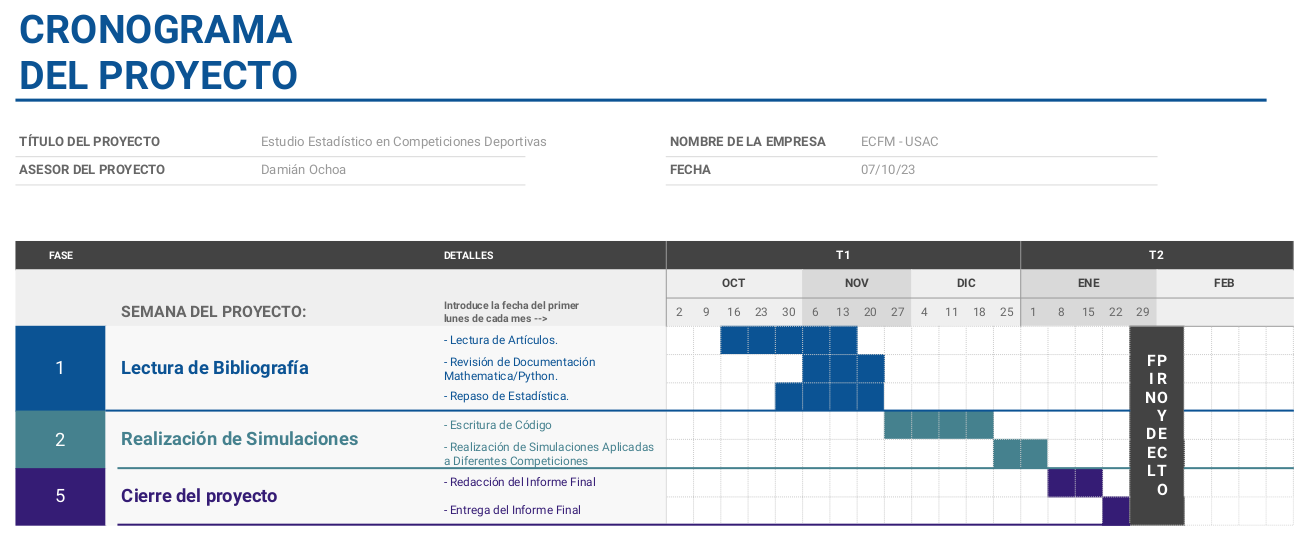
\includegraphics[scale=0.35]{./img/diagramaGantt.png}
	\caption{Diagrama de Gantt del Proyecto}
	\label{gantt}
\end{figure}


%\begin{thebibliography}{00}
%\bibitem{b1} Falomir, H. (2015). \textit{Curso de métodos de la física matemática.} Series: Libros de Cátedra.
%\bibitem{b2} Saxe, K. (2002). \textit{Beginning functional analysis (p. 7)}. New York: Springer.
%\bibitem{b3} Reed, M. (2012). \textit{Methods of modern mathematical physics: Functional analysis.} Elsevier.
%\bibitem{b4} Axler, S. (2015). \textit{Linear algebra done right.} springer publication.
%\bibitem{b5} Bartle, R. G., \& Sherbert, D. R. (2000). \textit{Introduction to real analysis.} John Wiley \& Sons, Inc..
%\end{thebibliography}



\end{titlepage}
\end{document}
